\documentclass[tikz,border=3pt]{standalone}
\usepackage[utf8]{inputenc}
\usepackage[T1]{fontenc}
\usepackage{lmodern}
\renewcommand{\familydefault}{\sfdefault}
\usepackage{sansmath}\sansmath
\usepackage{chemfig}
\usepackage{pgfplots}\pgfplotsset{compat=1.18,/pgf/number format/use comma,/pgf/number format/1000 sep={.}}
\usetikzlibrary{arrows.meta,calc,positioning,decorations.pathmorphing,patterns}
% paleta del sitio
\definecolor{nar}{HTML}{E8680C}\definecolor{narc}{HTML}{FFB35C}\definecolor{hielo}{HTML}{FFF3E8}
\definecolor{tinta}{HTML}{1D1D1F}\definecolor{gris}{HTML}{6E6E73}\definecolor{lila}{HTML}{7C5CF0}
\definecolor{azul}{HTML}{2F6FD6}\definecolor{menta}{HTML}{17A673}\definecolor{coral}{HTML}{E8342A}
\begin{document}
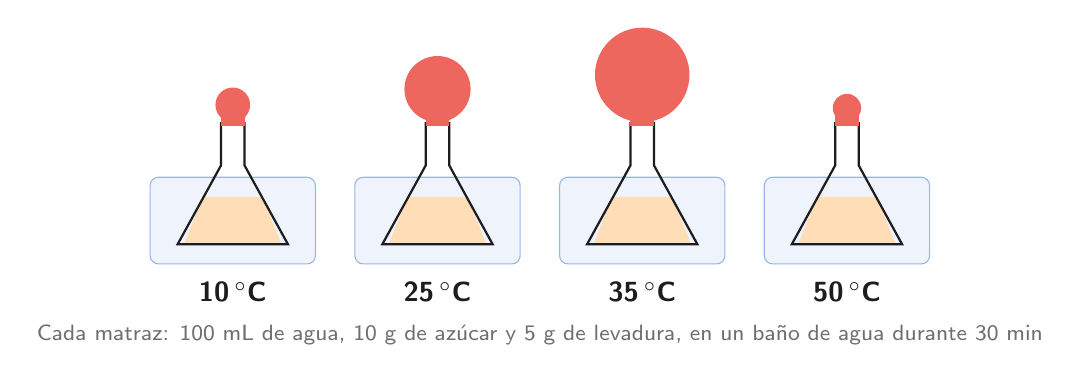
\begin{tikzpicture}[font=\small]
\foreach \i/\t/\r in {1/10/0.22,2/25/0.42,3/35/0.6,4/50/0.18}{
 \begin{scope}[shift={({2.6*(\i-1)},0)}]
  \fill[azul!8,rounded corners=3pt] (-1.05,-0.25) rectangle (1.05,0.85);
  \draw[azul!50,rounded corners=3pt] (-1.05,-0.25) rectangle (1.05,0.85);
  \fill[narc!45] (-0.62,0) -- (0.62,0) -- (0.38,0.6) -- (-0.38,0.6) -- cycle;
  \draw[tinta,thick] (-0.15,1.55) -- (-0.15,1.0) -- (-0.7,0) -- (0.7,0) -- (0.15,1.0) -- (0.15,1.55);
  \fill[coral!75] (0,{1.55+\r}) circle (\r);
  \fill[coral!75] (-0.15,1.5) rectangle (0.15,{1.6+0.2*\r});
  \node[text=tinta,font=\bfseries] at (0,-0.6) {\t\,$^\circ$C};
 \end{scope}}
\node[text=gris,font=\footnotesize] at (3.9,-1.15) {Cada matraz: 100 mL de agua, 10 g de azúcar y 5 g de levadura, en un baño de agua durante 30 min};
\end{tikzpicture}
\end{document}
